\documentclass{scrartcl}
\usepackage[utf8]{inputenc}
\usepackage[british]{babel}
\usepackage[T1]{fontenc}

\parindent 0pt
\parskip 0.5em

\usepackage[backend=bibtex8]{biblatex}
\bibliography{Handin}

\title{Assignment 7}
\author{Jakob Wittmann\\Dominik Schmidt}
\date{\today}

\usepackage{hyperref}
\usepackage[all]{hypcap}
\hypersetup{pdfborder = {0 0 0}, colorlinks=true, allcolors=black, urlcolor=blue}
\usepackage[margin=2.5cm]{geometry}
\usepackage{booktabs}
\usepackage{array}
\setlength{\tabcolsep}{.3em}

\usepackage{float}
\usepackage[export]{adjustbox}
\usepackage{amsmath}
\usepackage{listings}
\lstset{basicstyle=\ttfamily,breaklines=true}
\def\dd{\mathrm{d}}
\def\ml{\mathrm{\frac{mmol}{h}}}

\usepackage{longtable}
\usepackage{tikz}

\usepackage{enumitem}
\setlist[enumerate]{label=\alph*), labelsep=*}

\usepackage[version=4]{mhchem}

\begin{document}
\maketitle
\section{Growth coupling via knockouts}
\section{Production of a non-native compound}
	We consider the following pathway as suggested by \cite{BORODINA201557}, i.e. 
	\begin{figure}[h]
		\centering
		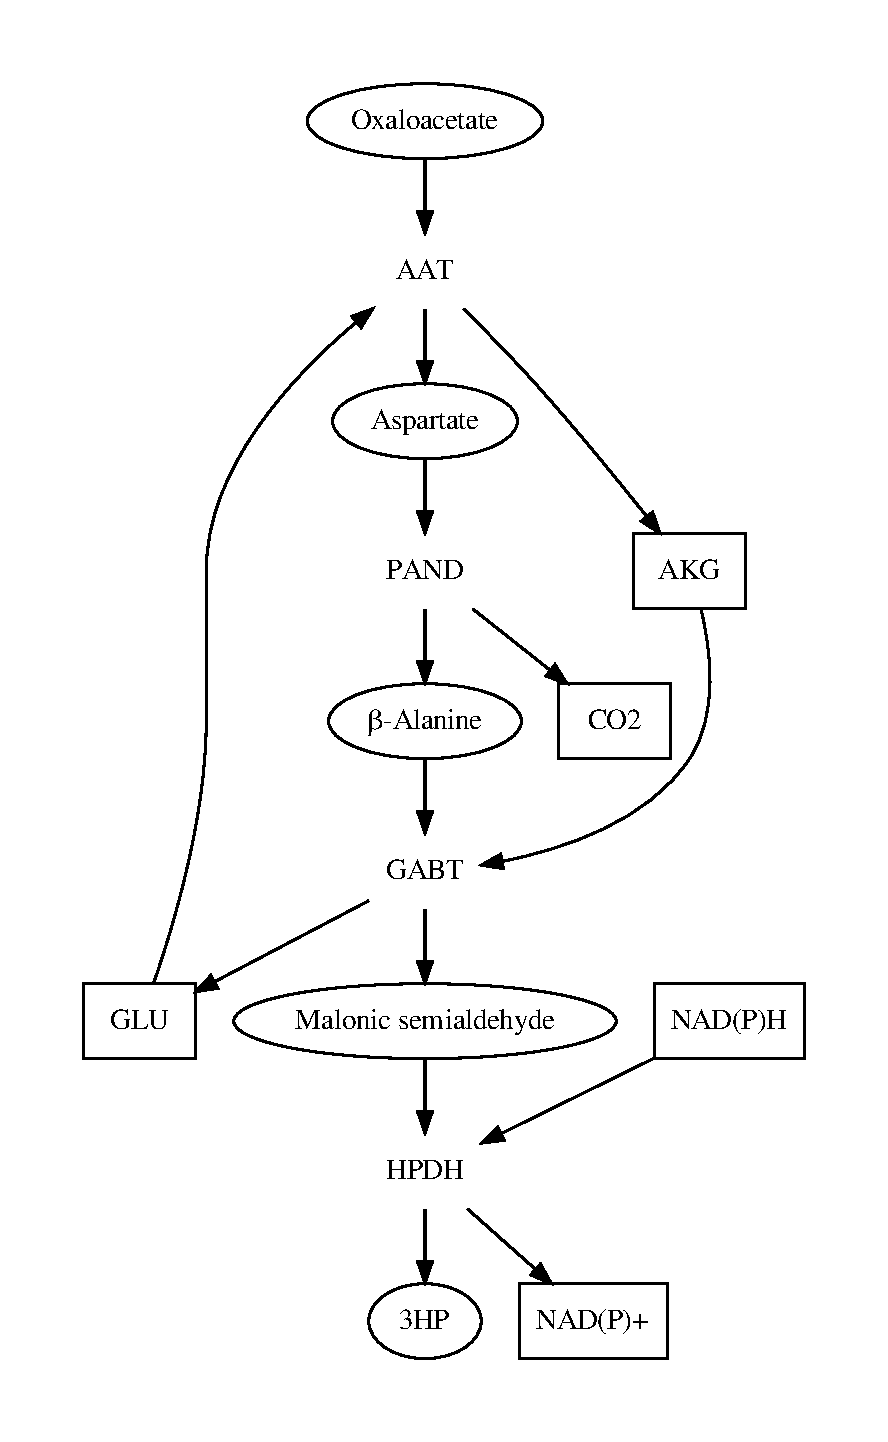
\includegraphics[max width=\linewidth, max height=0.74\paperheight]{2/new_pathway.pdf}
		\caption{The pathway to be added}
	\end{figure}
	We require the following additional metabolites:
	\begin{itemize}
		\item Aspartate, asp\_c
		\item $\beta$-Alanine, ala\_c
		\item Malonic Semaldehyde (3-Oxopropanoate), oxo\_c
		\item 3HP, hpa\_c
		\item 3HP, hpa\_e
		\item L-Glutamate, glu\_c
	\end{itemize}
	and the following reactions:
	\begin{align}
		oaa\_c + glu\_c &\rightarrow asp\_c + akg\_c \\
		asp\_c &\rightarrow ala\_c + co2\_c\\
		ala\_c + akg\_c &\rightarrow oxo\_c + glu\_c\\
		oxo\_c + nadph\_c &\rightarrow hpa\_c + nadp\_c\\
		hpa\_c &\rightarrow hpa\_e
	\end{align}
\section{Flux modulation}

\printbibliography
\end{document}
